\section{特性介绍}
\label{sec:features}

\begin{frame}
  \begin{center}
    \Huge{\textcolor{red}{特性介绍}}
  \end{center}
\end{frame}

\subsection{源码构建}

\begin{frame}[fragile]{一键安装:基于CMake}
  \begin{python}
$ curl -fsSL https://raw.github.com/ccup/cctest/master/install.sh | sh
  \end{python}
\end{frame}

\begin{frame}[fragile]{源码安装:CMake}
\begin{python}
$ mkdir build && cd build
$ cmake ..
$ make
$ make test
\end{python}
\end{frame}

\begin{frame}[fragile]{卸载:CMake}
\begin{python}
$ cat install_manifest.txt | xargs echo sudo rm | sh
\end{python}
\end{frame}

\begin{frame}[fragile]{源码构建:Bazel}
\begin{python}
$ bazel build //ctest
$ bazel build //ctest:main
\end{python}
\end{frame}

\subsection{破冰之旅}

\begin{frame}{需求:单位换算}
  \begin{enumerate}
    \item \textcolor{red}{1 FEET == 12 INCH}
    \item \textcolor{red}{1 YARD == 3 FEET}
    \item \textcolor{red}{1 MILE == 1760 YARD}
  \end{enumerate}
\end{frame}

\begin{frame}[fragile]{测试用例}
\begin{c++}
#include "quantity/length.h"
#include "cctest/cctest.h"

namespace {

FIXTURE(LengthTest) {
  TEST("1 feet == 12 inch") {
    ASSERT_EQ(Length(1, FEET), Length(12, INCH));
  }

  TEST("1 yard == 3 feets") {
    ASSERT_EQ(Length(1, YARD), Length(3, FEET));
  }

  TEST("1 mile == 1760 yards") {
    ASSERT_EQ(Length(1, MILE), Length(1760, YARD));
  }
};

} // namespace
\end{c++}
\end{frame}

\begin{frame}[fragile]{quantity/length.h}
\begin{c++}
#include "quantity/amount.h"

enum LengthUnit {
  INCH = 1,
  FEET = 12 * INCH,
  YARD = 3 * FEET,
  MILE = 1760 * YARD,
};

struct Length {
  Length(Amount amount, LengthUnit unit);

  bool operator==(const Length& rhs) const;
  bool operator!=const Length& rhs) const;

private:
  Amount amountInBaseUnit;
};
\end{c++}
\end{frame}

\begin{frame}[fragile]{quantity/length.cc}
\begin{c++}
#include "quantity/length.h"

Length::Length(Amount amount, LengthUnit unit)
  : amountInBaseUnit(unit * amount) {
}

bool Length::operator==(const Length& rhs) const {
  return amountInBaseUnit == rhs.amountInBaseUnit;
}

bool Length::operator!=(const Length& rhs) const {
  return !(*this == rhs);
}
\end{c++}
\end{frame}

\subsection{基本特性}

\begin{frame}{自我测试: cctest自己测试自己}
    \centering
    \begin{figure}
      \centering
      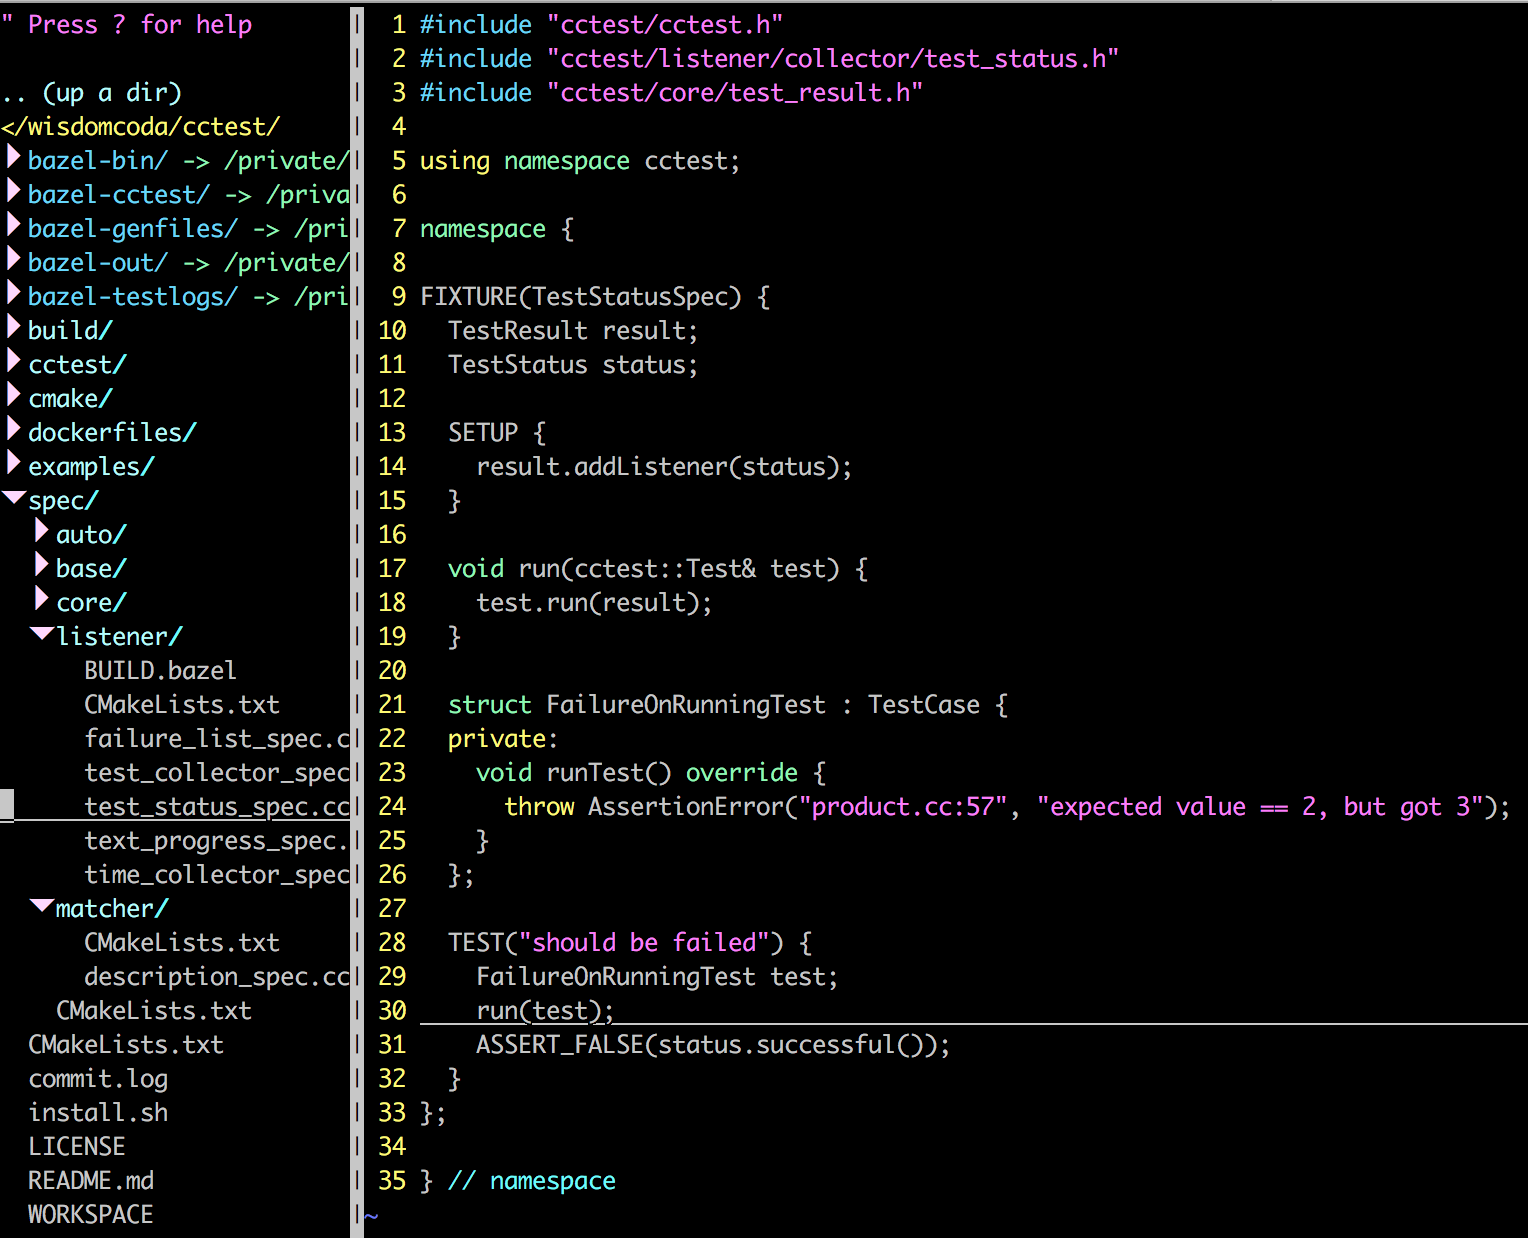
\includegraphics[width=0.7\textwidth]{test-status-spec.png}
    \end{figure}
\end{frame}

\begin{frame}{报表定制化}
    \centering
    \begin{figure}
      \centering
      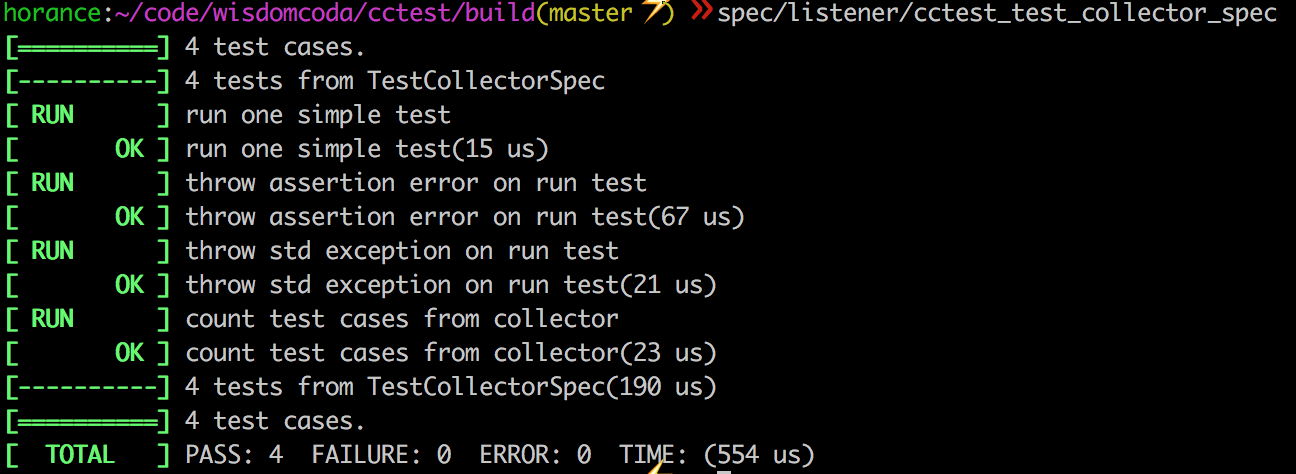
\includegraphics[width=1.0\textwidth]{color-printer.png}
    \end{figure}

    \begin{itemize}
    \item \alert{标准输出}:彩色终端,纯色终端
    \item \alert{CI/CD报表}:XML, JSON, YAML
    \end{itemize}    
\end{frame}

\begin{frame}{构建系统: Bazel}
    \centering
    \begin{figure}
      \centering
      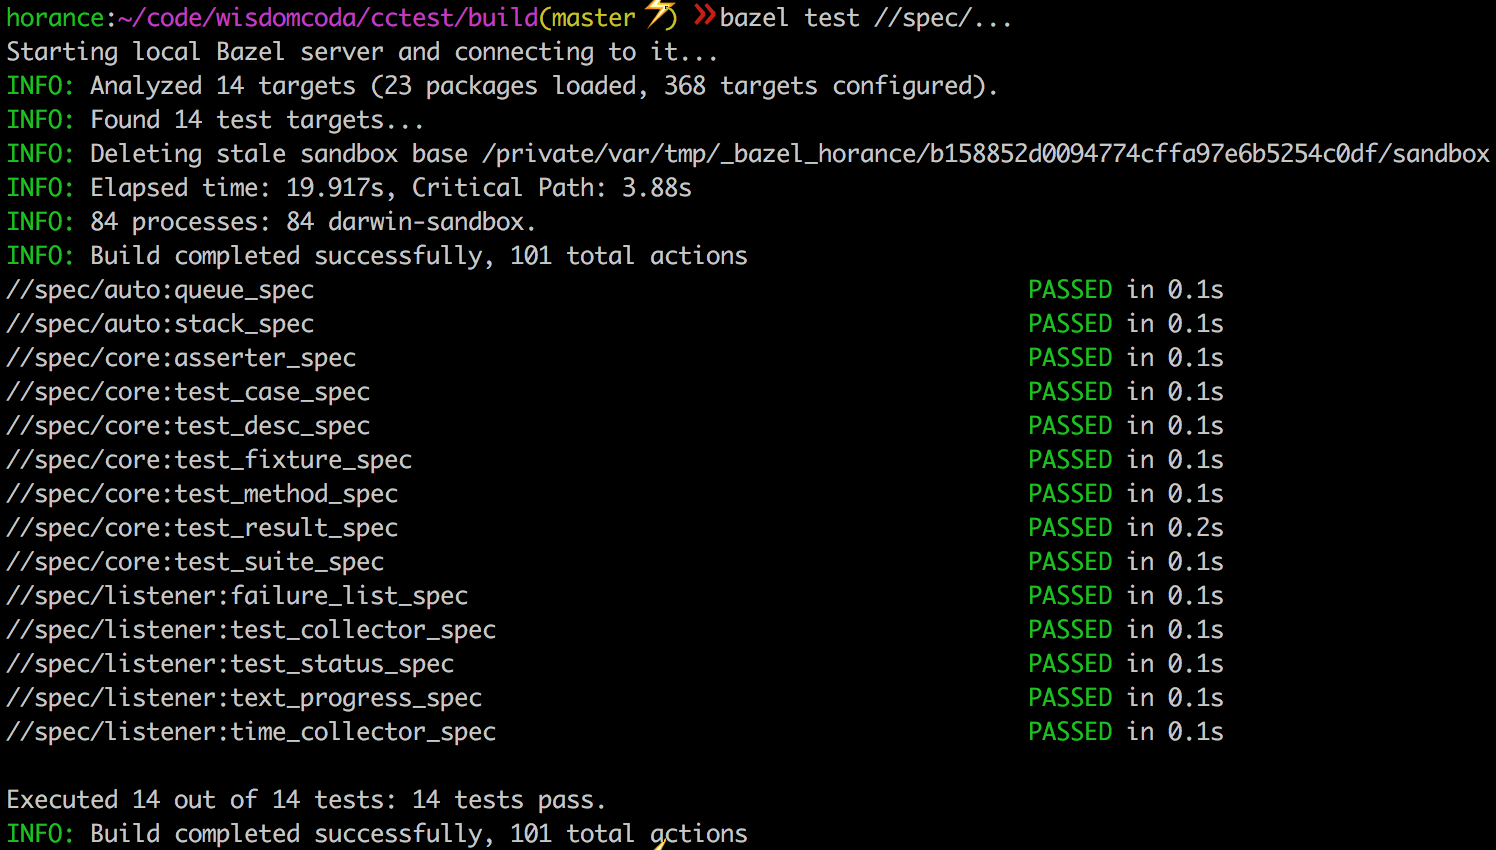
\includegraphics[width=0.9\textwidth]{test-in-bazel.png}
    \end{figure}
\end{frame}

\begin{frame}{构建系统: CMake}
    \centering
    \begin{figure}
      \centering
      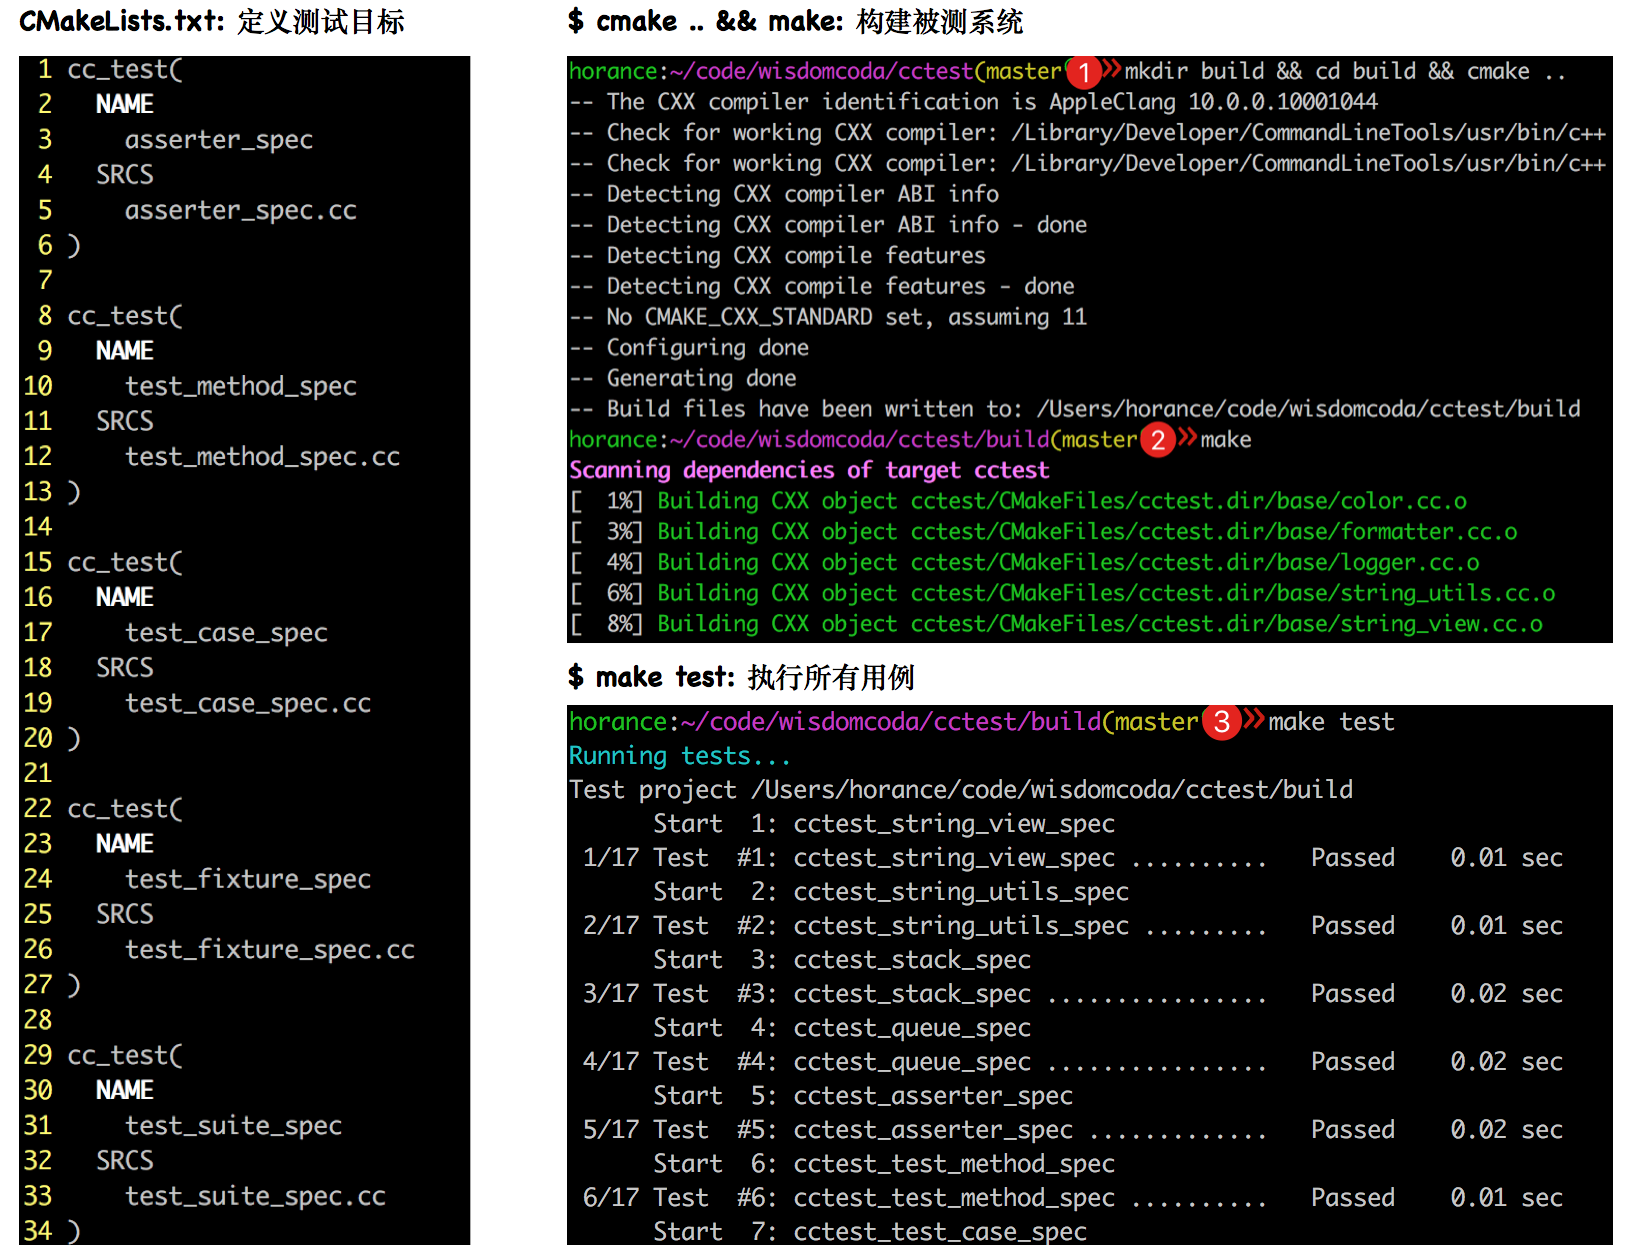
\includegraphics[width=0.9\textwidth]{test-in-cmake.png}
    \end{figure}
\end{frame}

\begin{frame}{Anotation语义}
  \begin{columns}
    \column{0.3\textwidth}
     \begin{block}{语义定制}
       \begin{enumerate}
         \item 测试依赖
         \item 超时检测
         \item 异常检测
         \item 执行数目 
         \item Tag标签过滤
         \item 内存溢出检测
       \end{enumerate}
     \end{block}

    \column{0.7\textwidth}
    \begin{figure}
      \centering
      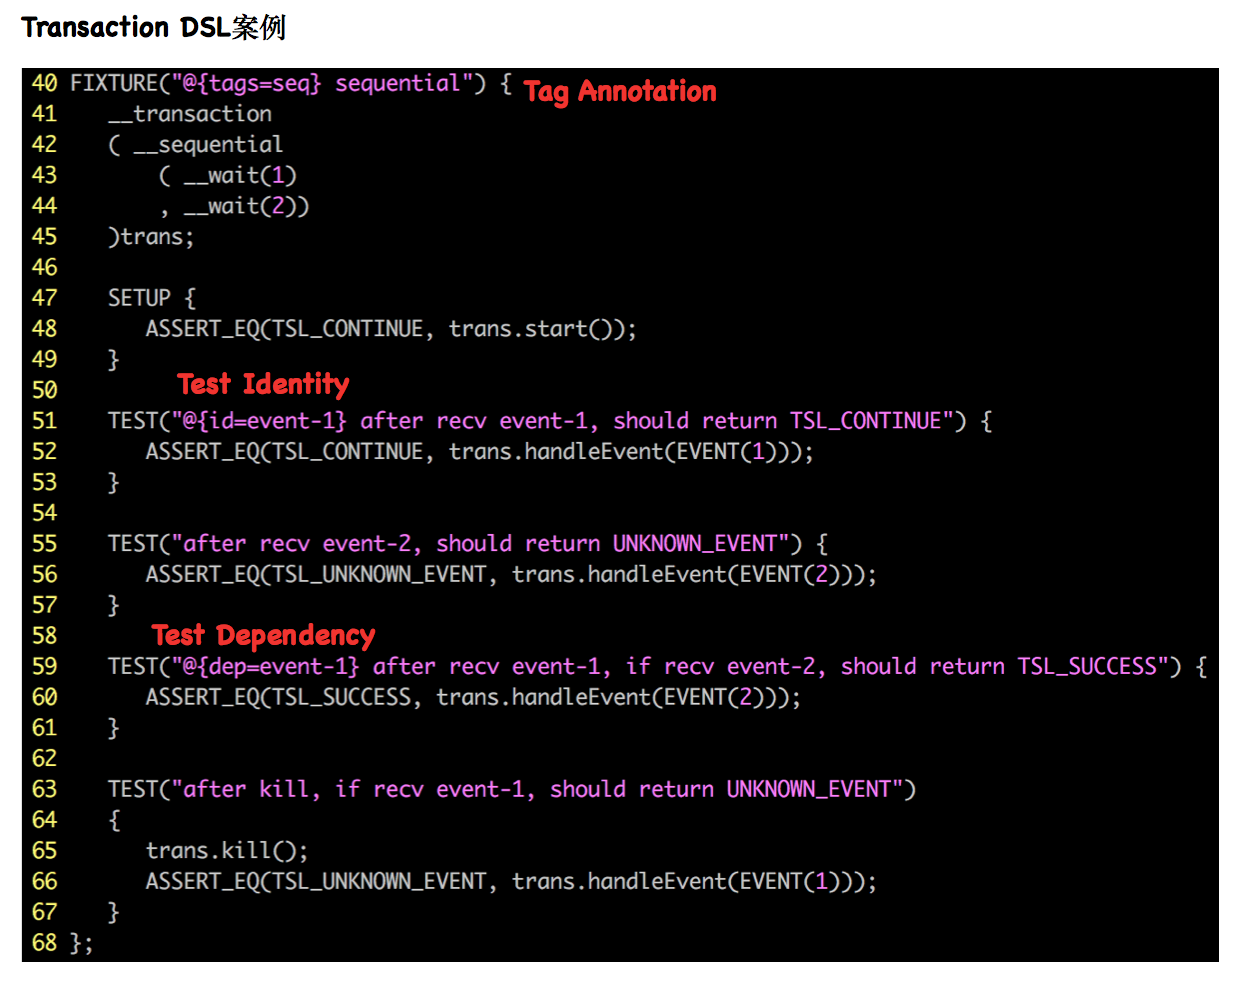
\includegraphics[width=1.0\textwidth]{trans-dsl.png}
    \end{figure}
  \end{columns}
\end{frame}

\begin{frame}{可扩展断言机制:ASSERT\_THAT \& 匹配器}
    \centering
    \begin{figure}
      \centering
      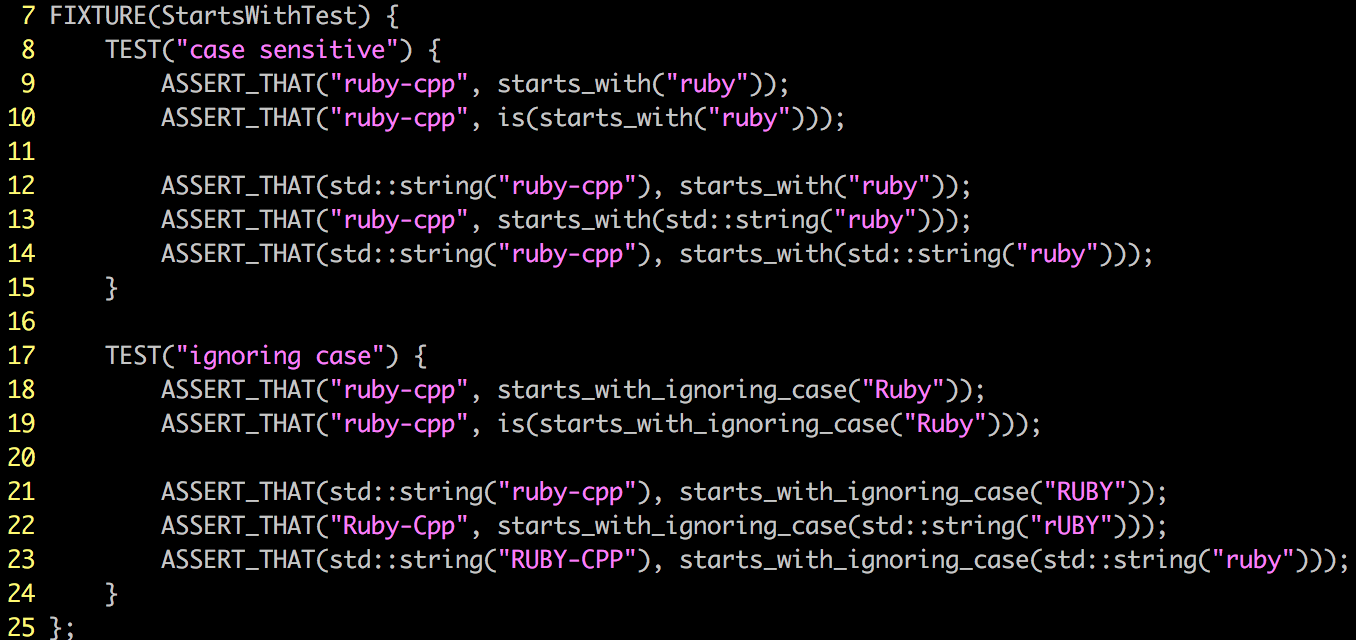
\includegraphics[width=1.0\textwidth]{macher-starts-with.png}
    \end{figure}
\end{frame}
